\section {Testing}
\paragraph{}
Testing was used to ensure the robustness of the solution, guaranteeing that all the project's objectives were met successfully. Recall that the tests themselves were designed in section 2, with the intention of being carried out after the design had been fully implemented, and were grouped by which objective each aimed to test.

\paragraph{}
The auditory nature of the program means it is not possible to fully provide evidence of successful tests with only the written word. Screenshots are therefore included within the document for the benefit of the reader, as well as external video links containing both video and audio.

\paragraph{}
Naturally testing would not be complete without checking for the presence of errors. Recall therefore that the design of tests encompasses both boundary and erroneous data in addition to "normal data", particularly in the loading of playlists and audio files.

\paragraph{}
Evidence for each test follows the same basic structure:
\begin{itemize}
	\item Re-cap of test
	\item Supplied test data
	\item Expected result
	\item Observed result
	\item Conclusion: was the observed result as expected?
\end{itemize}

\paragraph{}
For the benefit of the reader, a summary of the results of all tests is contained below.
Below that are the tests themselves, expanded in more detail.

% Redefine \pageref to include "Page" before the page number
\newcommand{\fullpageref}[1]{\hyperref[{#1}]{Page~\pageref{#1}}}

\pagebreak
\subsection{Testing Summary}
{
	\renewcommand{\arraystretch}{1.5}
	\begin{table}[h!]
		\begin{center}
			\begin{tabularx}{1.0 \textwidth} {
					| >{\raggedright\arraybackslash}p{0.1\linewidth}
					| >{\raggedright\arraybackslash}X
					| >{\raggedright\arraybackslash}p{0.1\linewidth}
					|>{\raggedright\arraybackslash}p{0.1\linewidth}
					|
				}
				\hline
				Test Number & Description & Relevant Evidence & Passed \\

				\hline
				1.1 & "The user must have the option to create a new playlist from a list of audio files on the system.  To test this, I will therefore place a variety of audio files on disk and verify they are detected by the program. Non-audio files will not be able to be selected, for obvious reasons. As the only audio file currently supported is the ".wav" format, any file without this extension will not be displayed." & \fullpageref{sec:evidence1.1}& Yes\\

				\hline
				1.2 & "I will then test if playlists created in the program can be successfully saved to disk, then loaded back into the program in a sanitised manner. In other words, playlists consisting solely of files which actually exist on disk should be loaded without error (such that audio playback starts), but playlists with non-existent audio files should fail to load and notify the user of the error." & \fullpageref{sec:evidence1.2} & Yes\\

				\hline
				1.3 & "After loading a playlist and beginning audio playback, the audio files contained within must appear alphabetically in the audio file selection screen, ordered in ascending order by their respective filenames." & \fullpageref{sec:evidence1.3} & Yes\\

				\hline
				1.4 & "Any invalid audio files should be skipped over, and should not crash the program. The user should be notified if this happens." & \fullpageref{sec:evidence1.4} & Yes\\

				\hline
				2.1 & "A correct visualisation of a sine wave is apparent at 500 Hz, with a single peak corresponding to that frequency." & \fullpageref{sec:evidence2.1} & Yes\\

				\hline
				2.2 & "A correct visualisation of a sine wave is apparent at 1,000 Hz, with a single peak corresponding to that frequency." & \fullpageref{sec:evidence2.2} & Yes\\

				\hline
				2.3 & "Sine waves outside the human audible range, at 10 Hz and 30,000 Hz respectively, produce no visible output, as they are inaudible." & \fullpageref{sec:evidence2.3} & Yes\\

				\hline
				2.4 & "A correct visualisation of two sine waves (one at 1,000 Hz and one at 10,000 Hz) is apparent, with two separate peaks corresponding to those frequencies." & \fullpageref{sec:evidence2.4} & Yes\\

				\hline
				2.5 & "A correct visualisation of three sine waves (1,000 Hz, 5,000 Hz and 15,000 Hz ) is apparent, with three separate peaks corresponding to those frequencies." & \fullpageref{sec:evidence2.5} & Yes\\

				\hline
				3.1 & "The program's equaliser effect is able to selectively reduce the bass of any given audio (corresponding to the low frequencies in frequency space)." & \fullpageref{sec:evidence3.1} & Yes\\

				\hline
				3.2 & "The program's equaliser effect is able to selectively reduce the treble of any given audio (corresponding to the high frequencies in frequency space)." & \fullpageref{sec:evidence3.2} & Yes\\

				\hline
			\end{tabularx}
		\end{center}
	\end{table}
}
\pagebreak
{
	\renewcommand{\arraystretch}{1.5}
	\begin{table}[h!]
		\begin{center}
			\begin{tabularx}{1.0 \textwidth} {
					| >{\raggedright\arraybackslash}p{0.1\linewidth}
					| >{\raggedright\arraybackslash}X
					| >{\raggedright\arraybackslash}p{0.1\linewidth}
					|>{\raggedright\arraybackslash}p{0.1\linewidth}
					|
				}
				\hline
				Test Number & Description & Relevant Evidence & Passed \\

				\hline
				4.1 & "A select group from the target audience certify that the echo effect sounds physically plausible, and mimics the effect as it is commonly heard in song remixes" & \fullpageref{sec:evidence4.1} & Yes\\

				\hline
				4.2 & "A select group from the target audience certify that the noise effect sounds physically plausible, and mimics the effect as it is commonly heard in song remixes" & \fullpageref{sec:evidence4.2} & Yes\\

				\hline
				4.3 & "The volume effect can be seen to adjust the volume correctly" & \fullpageref{sec:evidence4.3} & Yes\\

				\hline
				5.1 & "The noise effect can have its various parameters modified, which results in a correct change in the audio playback." & \fullpageref{sec:evidence5.1} & Yes\\

				\hline
				5.2 & "The echo effect can have its various parameters modified, which results in a correct change in the audio playback." & \fullpageref{sec:evidence5.2} & Yes\\

				\hline
				5.3 & "The equaliser effect can have its various parameters modified, which results in a correct change in the audio playback." & \fullpageref{sec:evidence5.3} & Yes\\

				\hline
				5.4 & "All presets present in the application can be loaded successfully, with the appropriate audio effects having been added and configured correctly, such that the desired effect is reached." & \fullpageref{sec:evidence5.4} & Yes\\
				
				\hline
				6.1 & "The program must run, without any effects applied, in real-time on the specified hardware." & \fullpageref{sec:evidence6} & Exceeded\\
				
				\hline
				6.2 & "The program must run in real-time, with every effect applied at once, in real-time on the specified hardware." & \fullpageref{sec:evidence6} & Exceeded\\

				\hline
			\end{tabularx}
		\end{center}
	\end{table}
}


\pagebreak
\subsection{Test 1.1}
\subsubsection*{Description}
\paragraph{}
{
	\centering
	\fbox{\begin{minipage}{15cm}
			"The user must have the option to create a new playlist from a list of audio files on the system.  To test this, I will therefore place a variety of audio files on disk and verify they are detected by the program. Non-audio files will not be able to be selected, for obvious reasons. As the only audio file currently supported is the ".wav" format, any file without this extension will not be displayed."
	\end{minipage}}
}

\subsubsection*{Supplied Test Data}
\paragraph{}
A variety of audio files were placed inside the system's music folder. Some were hidden inside subfolders. In order to test the behaviour of erroneous data as described above, the music folder also contained an mp3 file, which is not supported currently.

\begin{figure}[H]
	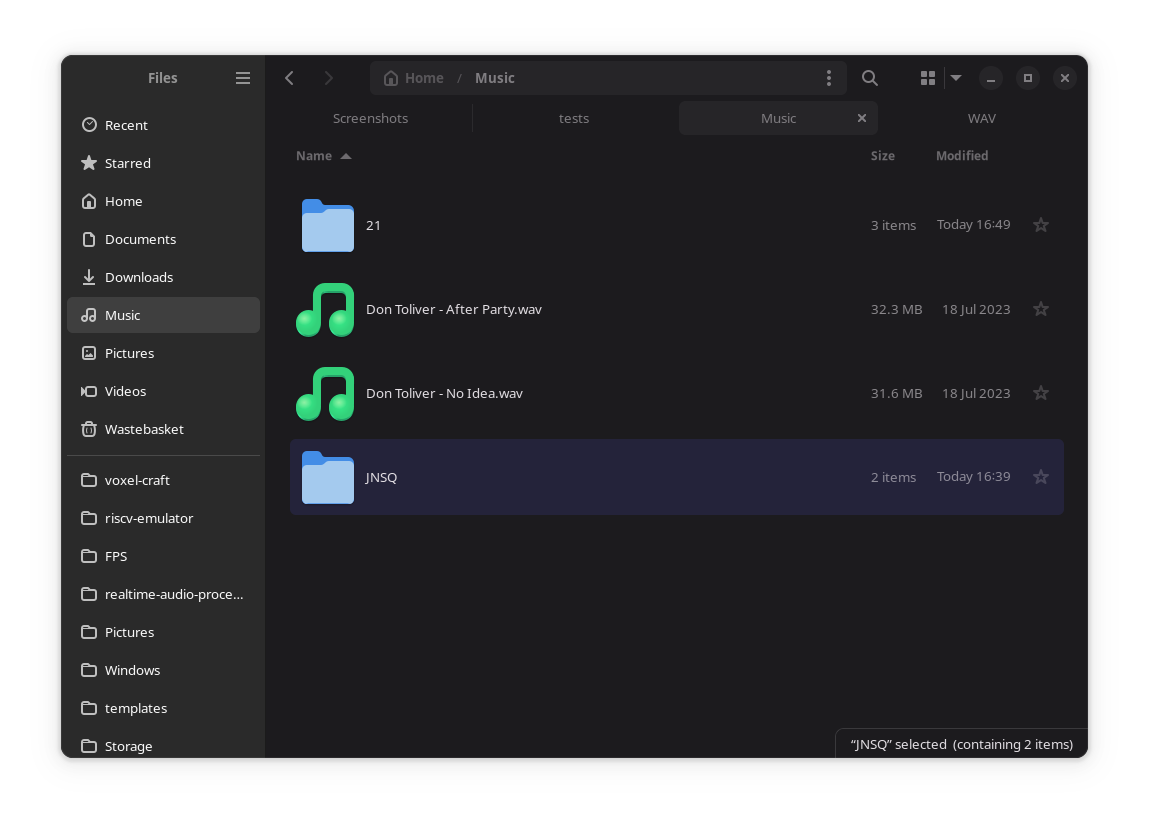
\includegraphics[width=14cm]{./tests/1.1.1.png}
\end{figure}
\begin{figure}[H]
	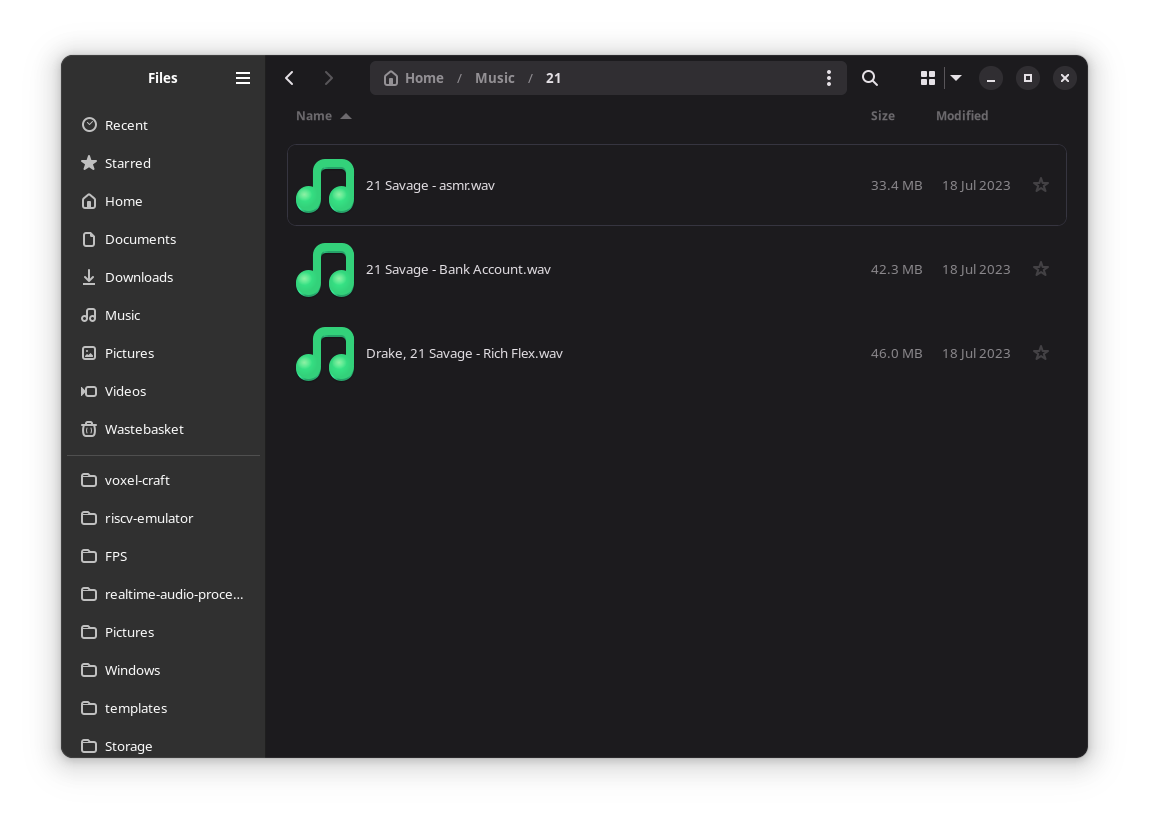
\includegraphics[width=14cm]{./tests/1.1.2.png}
\end{figure}
\begin{figure}[H]
	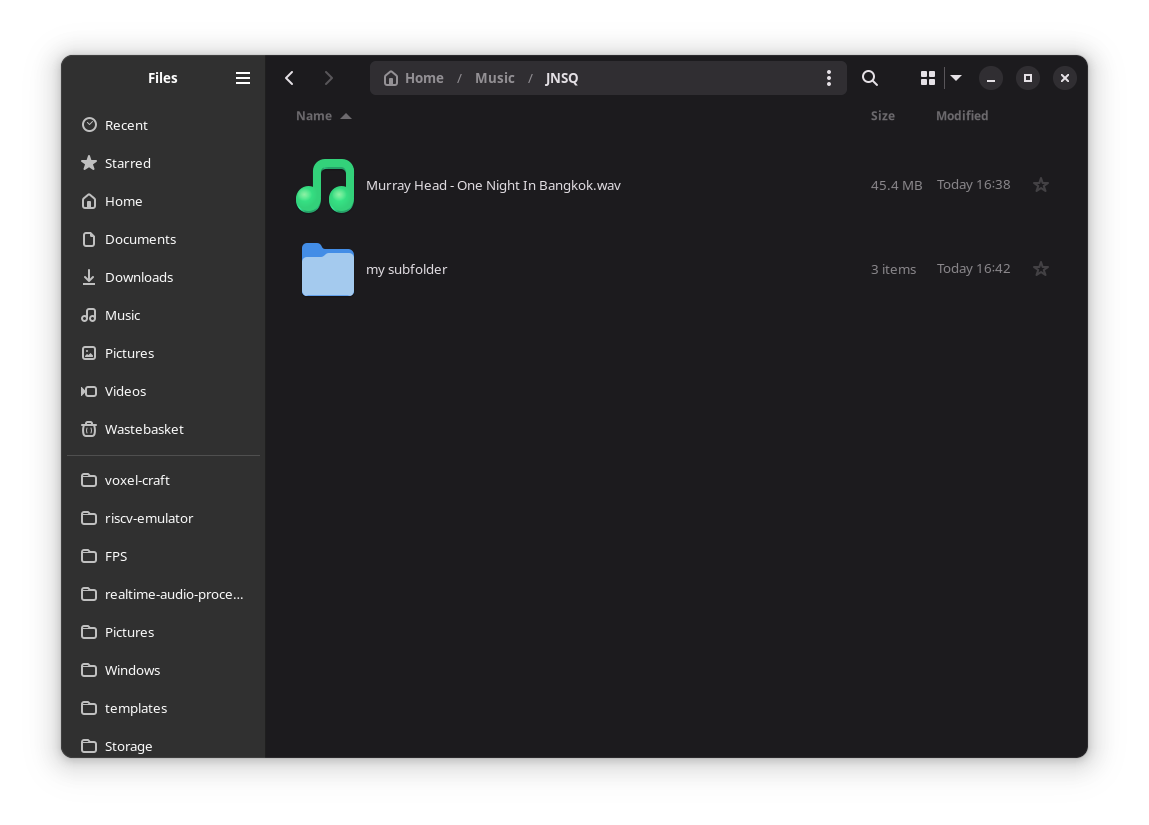
\includegraphics[width=14cm]{./tests/1.1.3.png}
\end{figure}
\begin{figure}[H]
	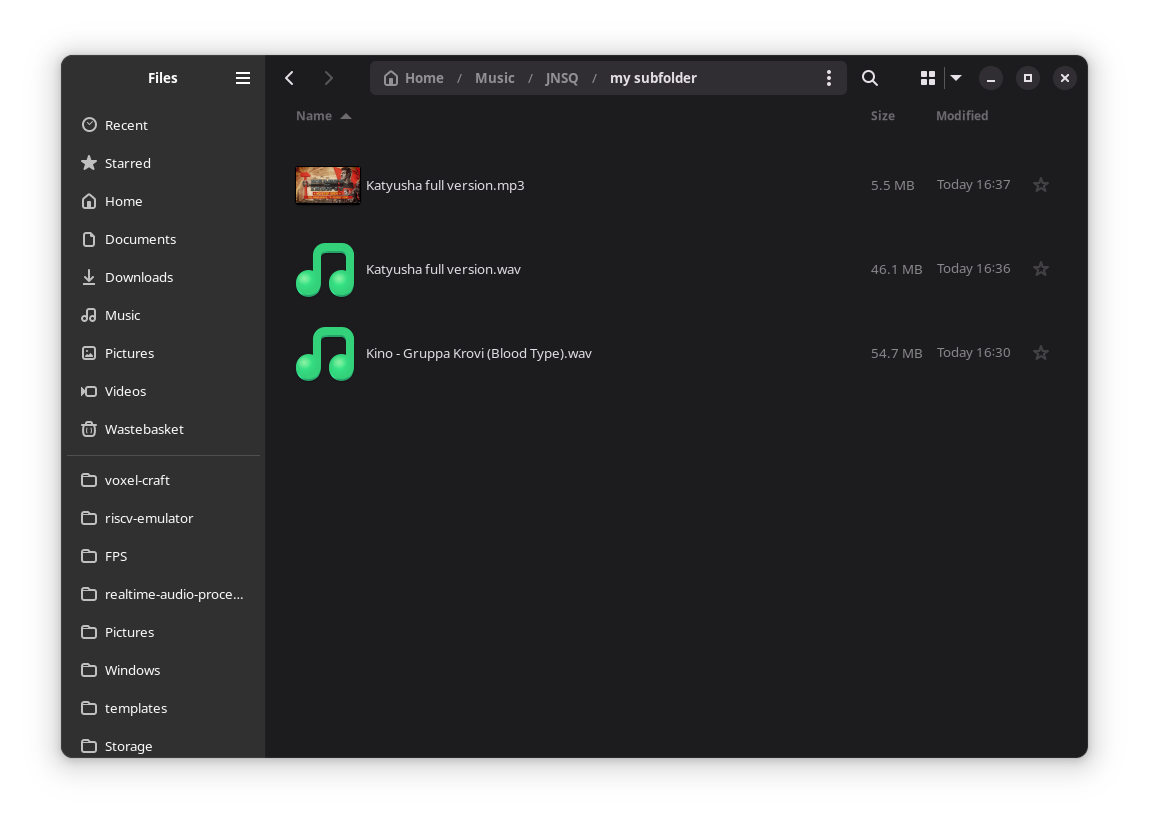
\includegraphics[width=14cm]{./tests/1.1.4.png}
\end{figure}
\begin{figure}[H]
	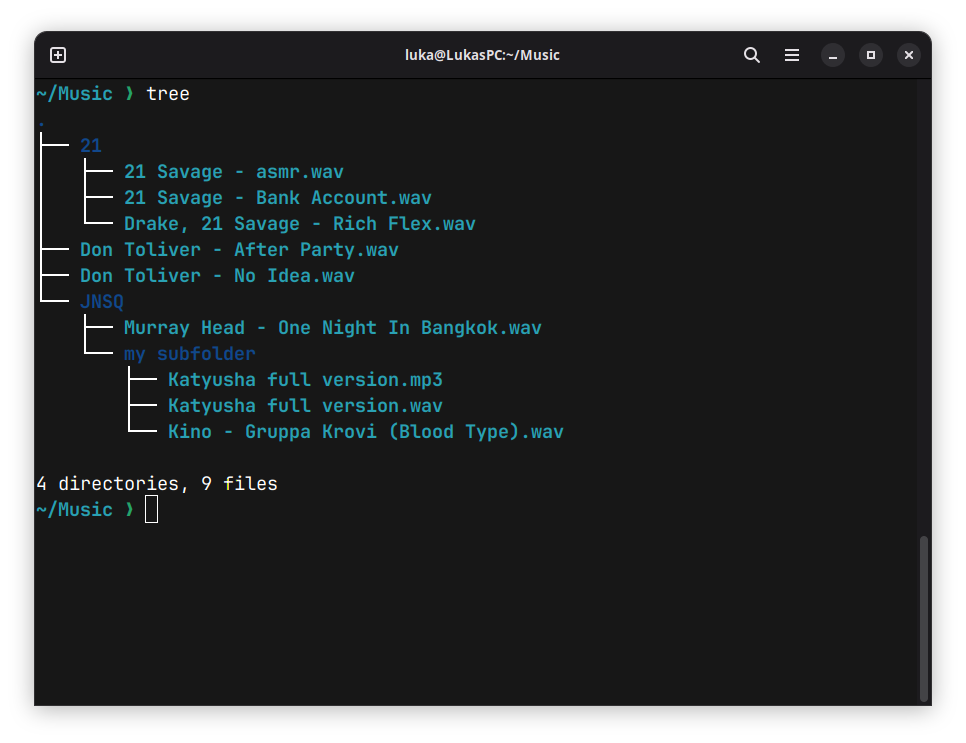
\includegraphics[width=14cm]{./tests/1.1.5.png}
	\caption{Terminal output that summarises filesystem structure}
\end{figure}

\subsubsection*{Expected Result}
The program should detect all the ".wav files", but not any other files, such that the ".mp3 file" is not detected. All detected files should be displayed within the GUI.

\subsubsection*{Observed Result}
\label{sec:evidence1.1}
\begin{figure}[H]
	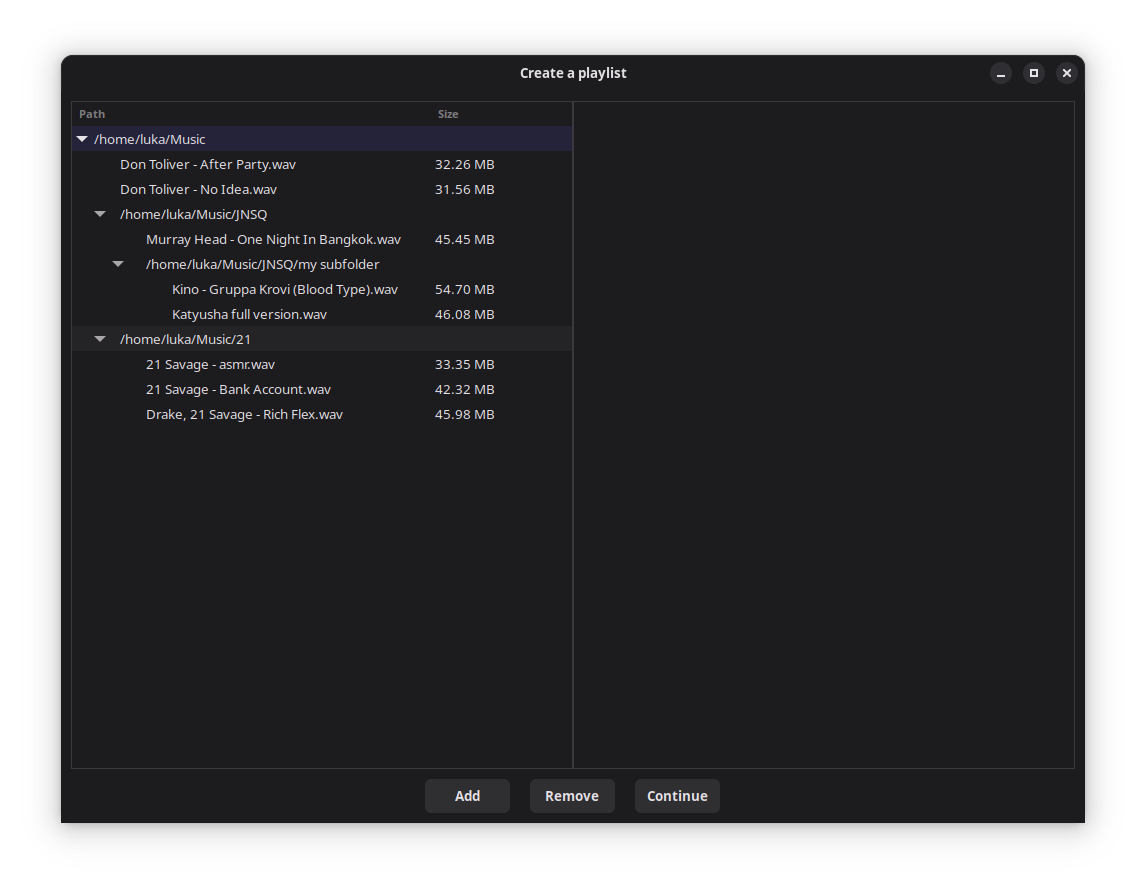
\includegraphics[width=14cm]{./tests/1.1.6.png}
	\caption{Program GUI output. All WAV files have been detected and displayed, but the mp3 has not been. Files have been detected, even when they are inside subfolders.}
\end{figure}

\subsubsection*{Conclusion}
This test passed, as all ".wav" audio files were detected, whilst other files were ignored, and the GUI displayed this appropriately.


\pagebreak
\subsection{Test 1.2}
\subsubsection*{Description}
\paragraph{}
{
	\centering
	\fbox{\begin{minipage}{15cm}
			"I will then test if playlists created in the program can be successfully saved to disk, then loaded back into the program in a sanitised manner. In other words, playlists consisting solely of files which actually exist on disk should be loaded without error (such that audio playback starts), but playlists with non-existent audio files should fail to load and notify the user of the error."
	\end{minipage}}
}

\subsubsection*{Supplied Test Data}
\paragraph{}
The test was split into two parts - the first would be attempting to create, save, then load a playlist in which all audio files existed. For the first part of this test, the same selection of files was used as in test 1.1. For the second part of the test, the playlist was to be modified after its creation by appending the following non-existent file to the end of it:
\textit{/this/audio/files/does/not/exist.wav}
\begin{figure}[H]
	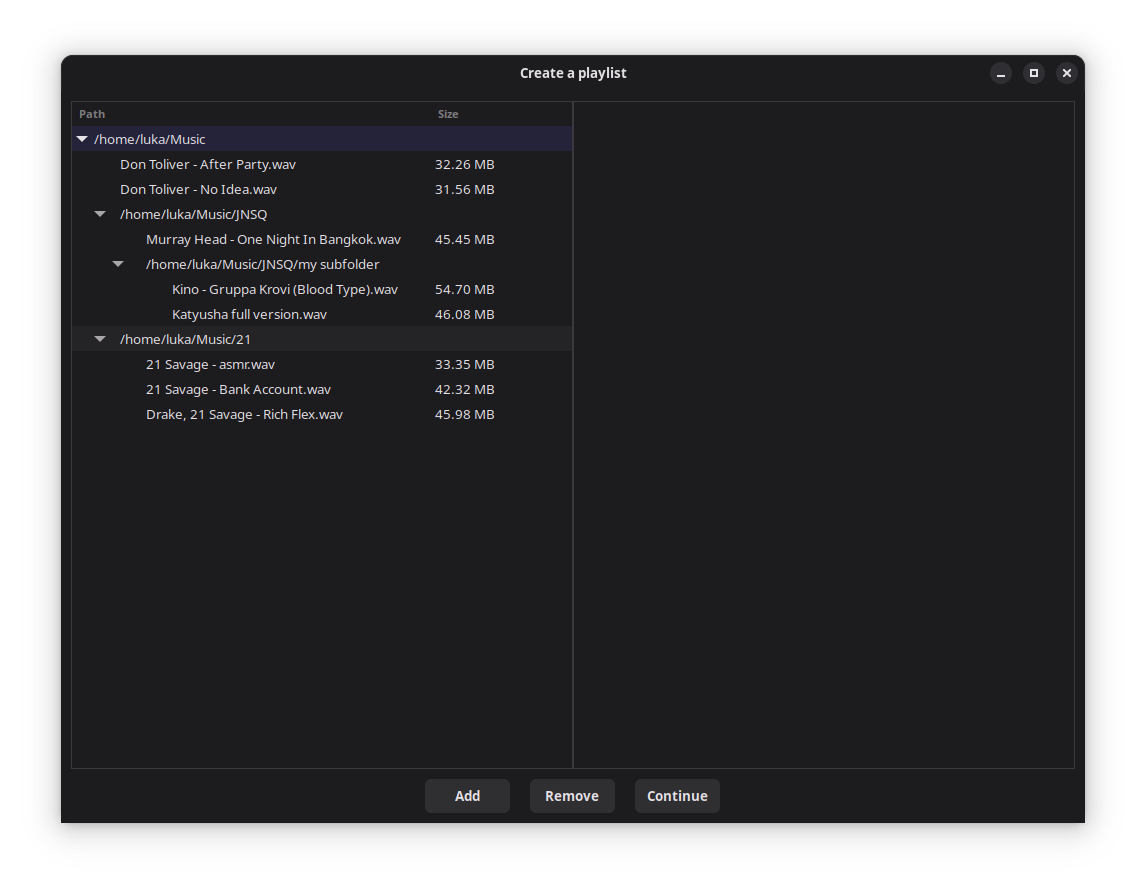
\includegraphics[width=14cm]{./tests/1.1.6.png}
	\caption{Files from test 1.1, which should be turned into a playlist then saved and loaded back}
\end{figure}

\subsubsection*{Expected Result}
The user should be able to use the GUI to add all files to a playlist, which is then saved successfully to disk. The user should then be able to load this playlist to begin audio playback. This should succeed. However, when the playlist is modified to include a file that no longer exists, the program should raise an error and refuse to load the playlist.

\subsubsection*{Observed Result}
\label{sec:evidence1.2}
Video evidence was recorded for the test, which can be viewed \href{https://drive.google.com/file/d/1yGeMYYI9ts37JsoA_9agpKTGBL0s8Dms/view?usp=sharing}{here}\footnote{
	https://drive.google.com/file/d/1yGeMYYI9ts37JsoA\_9agpKTGBL0s8Dms/view?usp=sharing
}.  The video shows a user created a valid playlist, then saving it to disk. He then loads the playlist into the program and audio playback successfully starts. He then restarts the program and attempts to load the playlist again, after modifying it by adding an invalid file path. The program refuses to load this invalid playlist.

\subsubsection*{Conclusion}
The program successfully created, saved, then loaded the valid playlist but refused to load the invalid playlist, such that the test passed.

\pagebreak
\subsection{Test 1.3}
\subsubsection*{Description}
\paragraph{}
{
	\centering
	\fbox{\begin{minipage}{15cm}
			"After loading a playlist and beginning audio playback, the audio files contained within must appear alphabetically in the audio file selection screen, ordered in ascending order by their respective filenames."
	\end{minipage}}
}

\subsubsection*{Supplied Test Data}
A new playlist was again created. It was deemed suitable as it contained audio files starting with upper case letters, lower case letters, and even numbers, hence allowing for all reasonable combinations of alpha-numeric values to be covered.
\begin{figure}[H]
	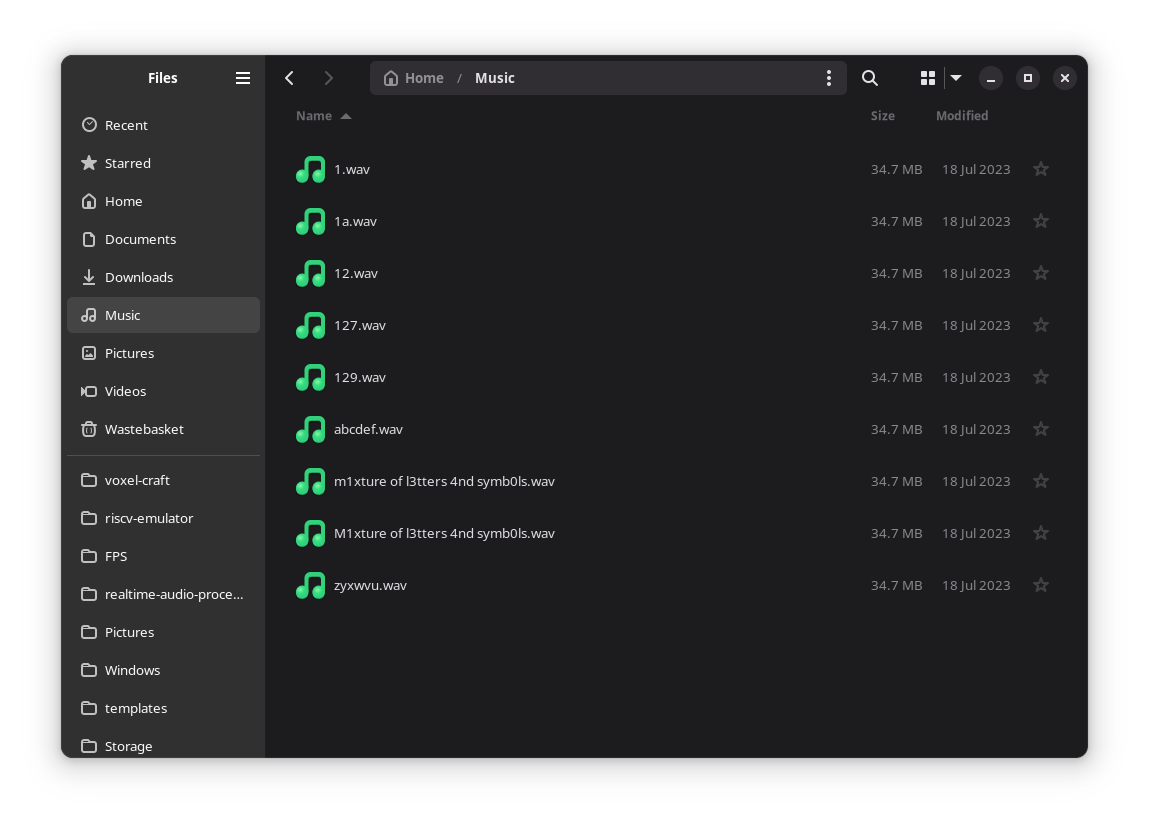
\includegraphics[width=14cm]{./tests/1.3.1.png}
\end{figure}

\subsubsection*{Expected Result}
\paragraph{}
When selecting a new audio file from the playlist (by going to \textit{File, Select Song}), the GUI should organise them alphabetically by their filenames. Numbers should come before letters, and the numbers should be ordered too (e.g, 1, 2, 3...). Lower case versions of the same letter should come before upper case versions (as they appear first in ASCII ordering).
\paragraph{}
Hence the expected order for display is as follows:
\begin{enumerate}
	\item 1.wav
	\item 1a.wav
	\item 12.wav
	\item 127.wav
	\item 129.wav
	\item abcdef.wav
	\item m1xture of l3tters 4nd symb0ls.wav
	\item M1xture of l3tters 4nd symb0ls.wav
	\item zyxwvu.wav
\end{enumerate}

\subsubsection*{Observed Result}
\label{sec:evidence1.3}
The observed result was as follows:
\begin{figure}[H]
	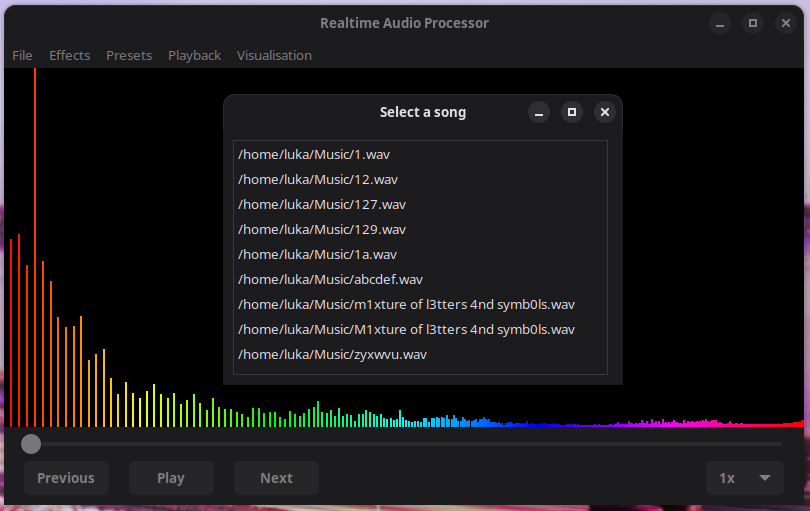
\includegraphics[width=14cm]{./tests/1.3.2.png}
\end{figure}

\subsubsection*{Conclusion}
The observed result and expected result were identical, such that the test passed.


\pagebreak
\subsection{Test 1.4}
\subsubsection*{Description}
\paragraph{}
{
	\centering
	\fbox{\begin{minipage}{15cm}
			"Any invalid audio files should be skipped over, and should not crash the program. The user should be notified if this happens."
	\end{minipage}}
}

\subsubsection*{Supplied Test Data}
A new playlist was again created, containing three files. The first and last files were valid audio files, but the middle one was corrupt. The playlist contained these three files:
\begin{figure}[H]
	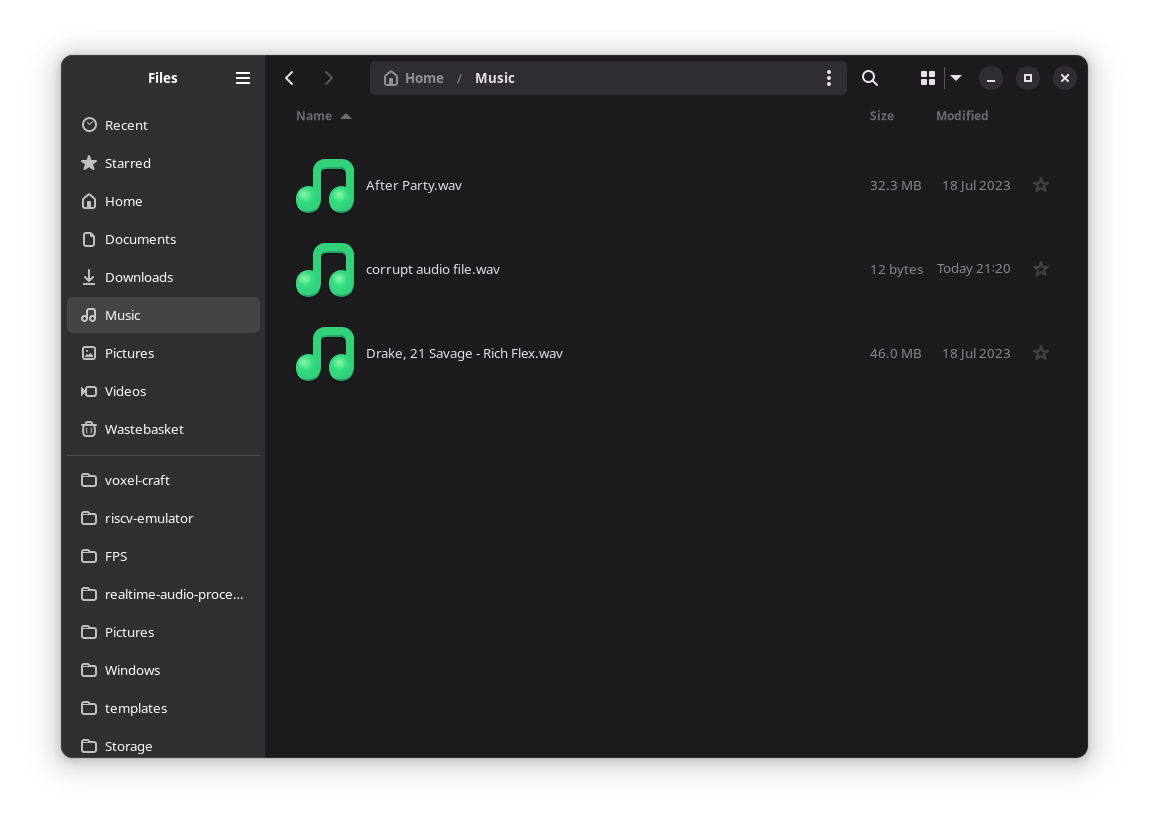
\includegraphics[width=14cm]{./tests/1.4.1.png}
\end{figure}

\subsubsection*{Expected Result}
\paragraph{}
The program should initially begin audio playback correctly when it loads the first audio file. However, when the next audio file (which is corrupt) is to be loaded by the program, it should fail, and the program should notify the user of the error. This corrupt file should then be skipped, and playback should resume with the third audio file.

\subsubsection*{Observed Result}
\label{sec:evidence1.4}
Video evidence was recorded for the test, which can be viewed \href{https://drive.google.com/file/d/1IWSDFYTCctY-Voe49W1-w-7M0zj7ucMX/view?usp=sharing}{here}\footnote{
	https://drive.google.com/file/d/1IWSDFYTCctY-Voe49W1-w-7M0zj7ucMX/view?usp=sharing
}.  The video shows a user loading the testing playlist, in which audio playback starts. They then skip to the end of the song, waiting for it to finish. When it does, the program attempts to load the next audio file (which the reader will recall is invalid). Naturally, the program catches this and raises an error to the user. This corrupt audio file is then skipped, and playback resumes with the next audio file.

\subsubsection*{Conclusion}
The observed result and expected result were identical, such that the test passed.

\pagebreak
\subsection{Test 2.1}
\subsubsection*{Description}
\paragraph{}
{
	\centering
	\fbox{\begin{minipage}{15cm}
			"A correct visualisation of a sine wave is apparent at 500 Hz, with a single peak corresponding to that frequency."
	\end{minipage}}
}

\subsubsection*{Supplied Test Data}
An audio file consisting of a single sine wave at 500 Hz was generated using the popular audio editing program Audacity.

\subsubsection*{Expected Result}
A single peak should be observed in the audio visualiser, towards the left of the screen, representing 500 Hz.

\subsubsection*{Observed Result}
\label{sec:evidence2.1}
\begin{figure}[H]
	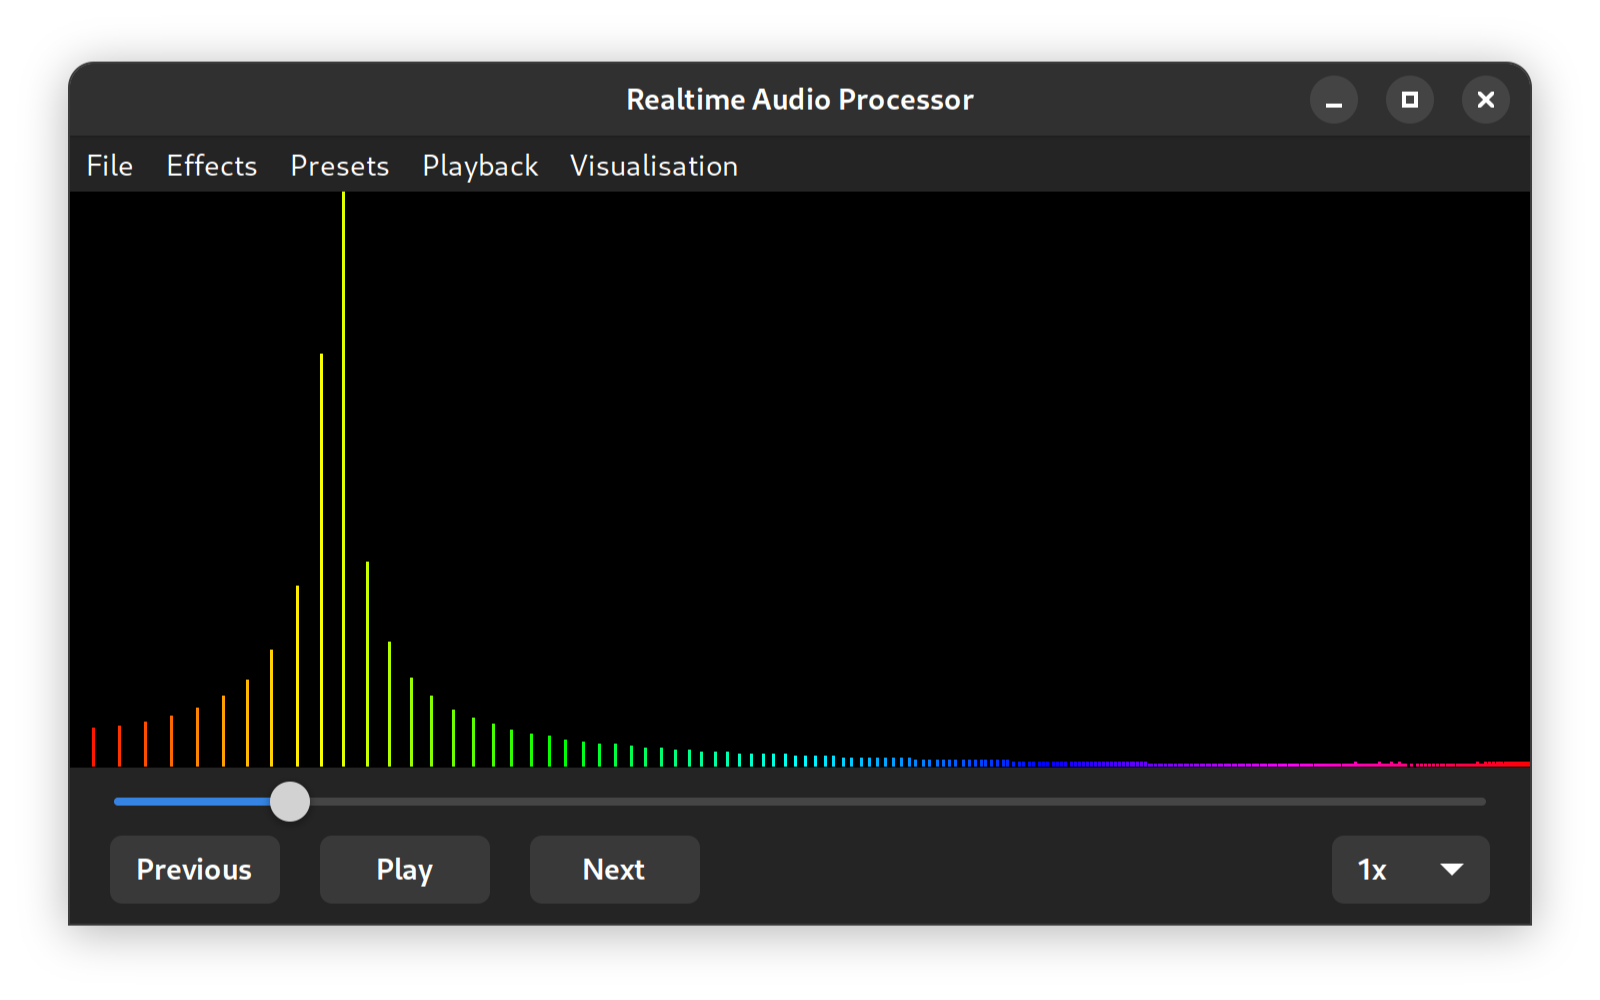
\includegraphics[width=14cm]{./tests/2.1.png}
\end{figure}

\subsubsection*{Conclusion}
A correct visualisation was achieved. The test was successful.

\pagebreak
\subsection{Test 2.2}
\subsubsection*{Description}
\paragraph{}
{
	\centering
	\fbox{\begin{minipage}{15cm}
			"A correct visualisation of a sine wave is apparent at 1,000 Hz, with a single peak corresponding to that frequency."
	\end{minipage}}
}

\subsubsection*{Supplied Test Data}
An audio file consisting of a single sine wave at 1,000 Hz was generated using the popular audio editing program Audacity.

\subsubsection*{Expected Result}
A single peak should be observed in the audio visualiser, to the right of the peak observed in Test 1.1 (as the frequency is higher).

\subsubsection*{Observed Result}
\label{sec:evidence2.2}
\begin{figure}[H]
	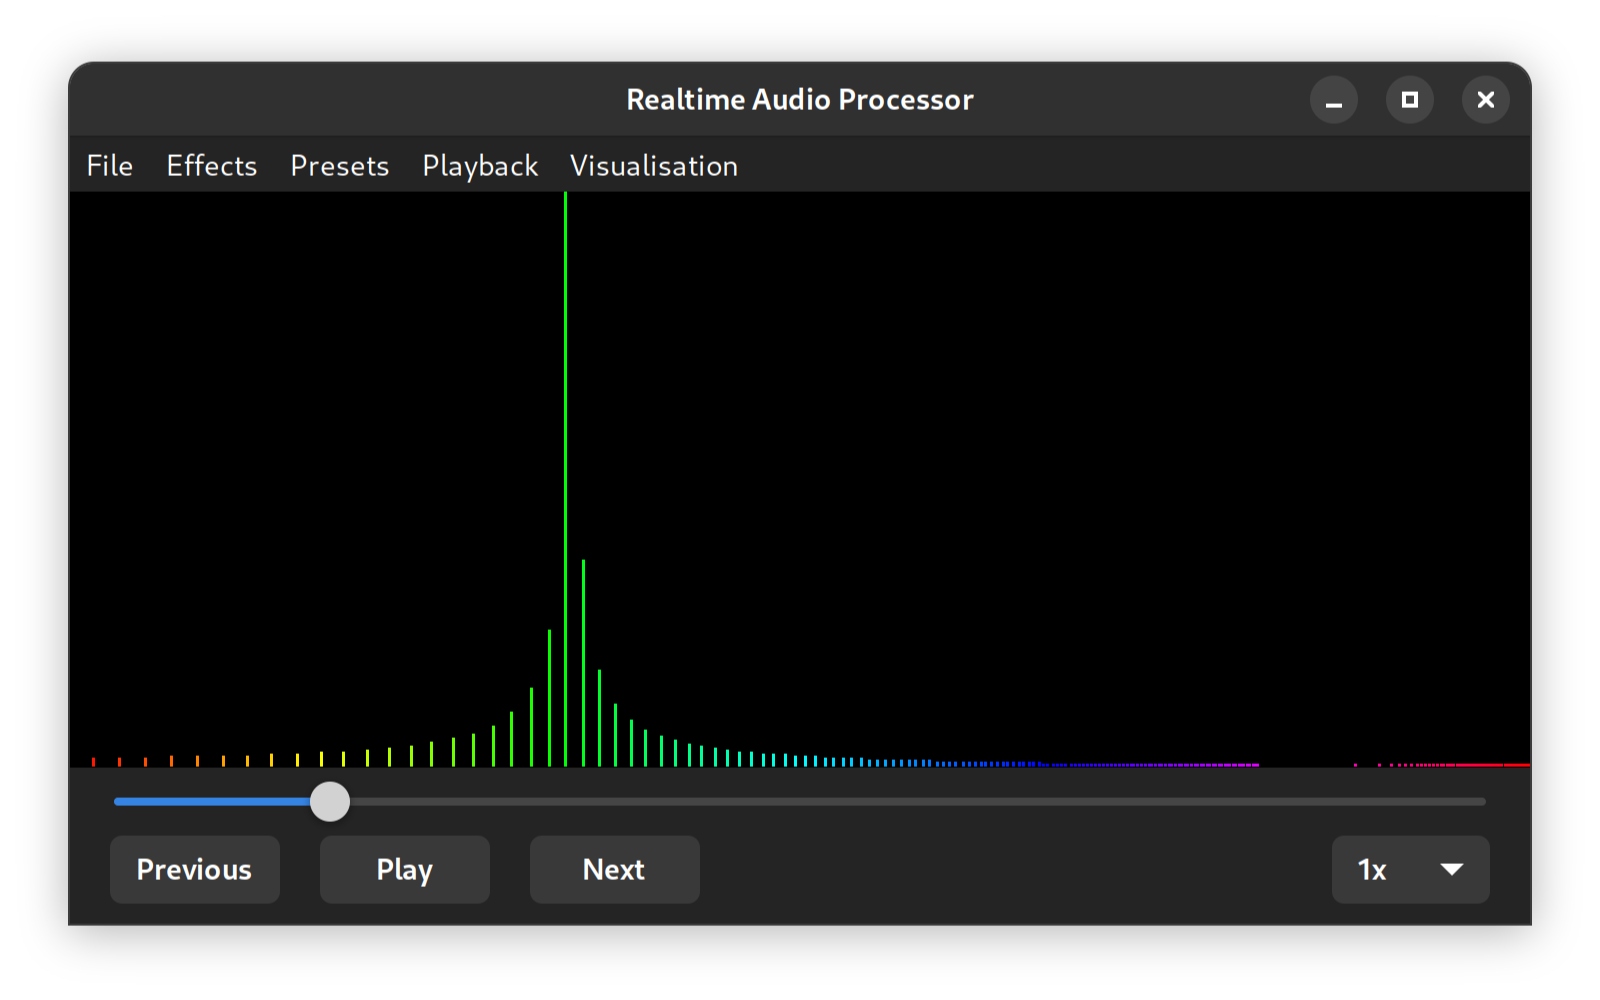
\includegraphics[width=14cm]{./tests/2.2.png}
\end{figure}

\subsubsection*{Conclusion}
A correct visualisation was achieved. The test was successful.

\pagebreak
\subsection{Test 2.3}
\subsubsection*{Description}
\paragraph{}
{
	\centering
	\fbox{\begin{minipage}{15cm}
			"Sine waves outside the human audible range, at 10 Hz and 30,000 Hz respectively, produce no visible output, as they are inaudible."
	\end{minipage}}
}

\subsubsection*{Supplied Test Data}
An audio file consisting of two sine waves (at 10 Hz and 30,000 Hz respectively) was generated using the popular audio editing program Audacity.

\subsubsection*{Expected Result}
The input audio is completely inaudible, so there should be no output in the visualiser.

\subsubsection*{Observed Result}
\label{sec:evidence2.3}
\begin{figure}[H]
	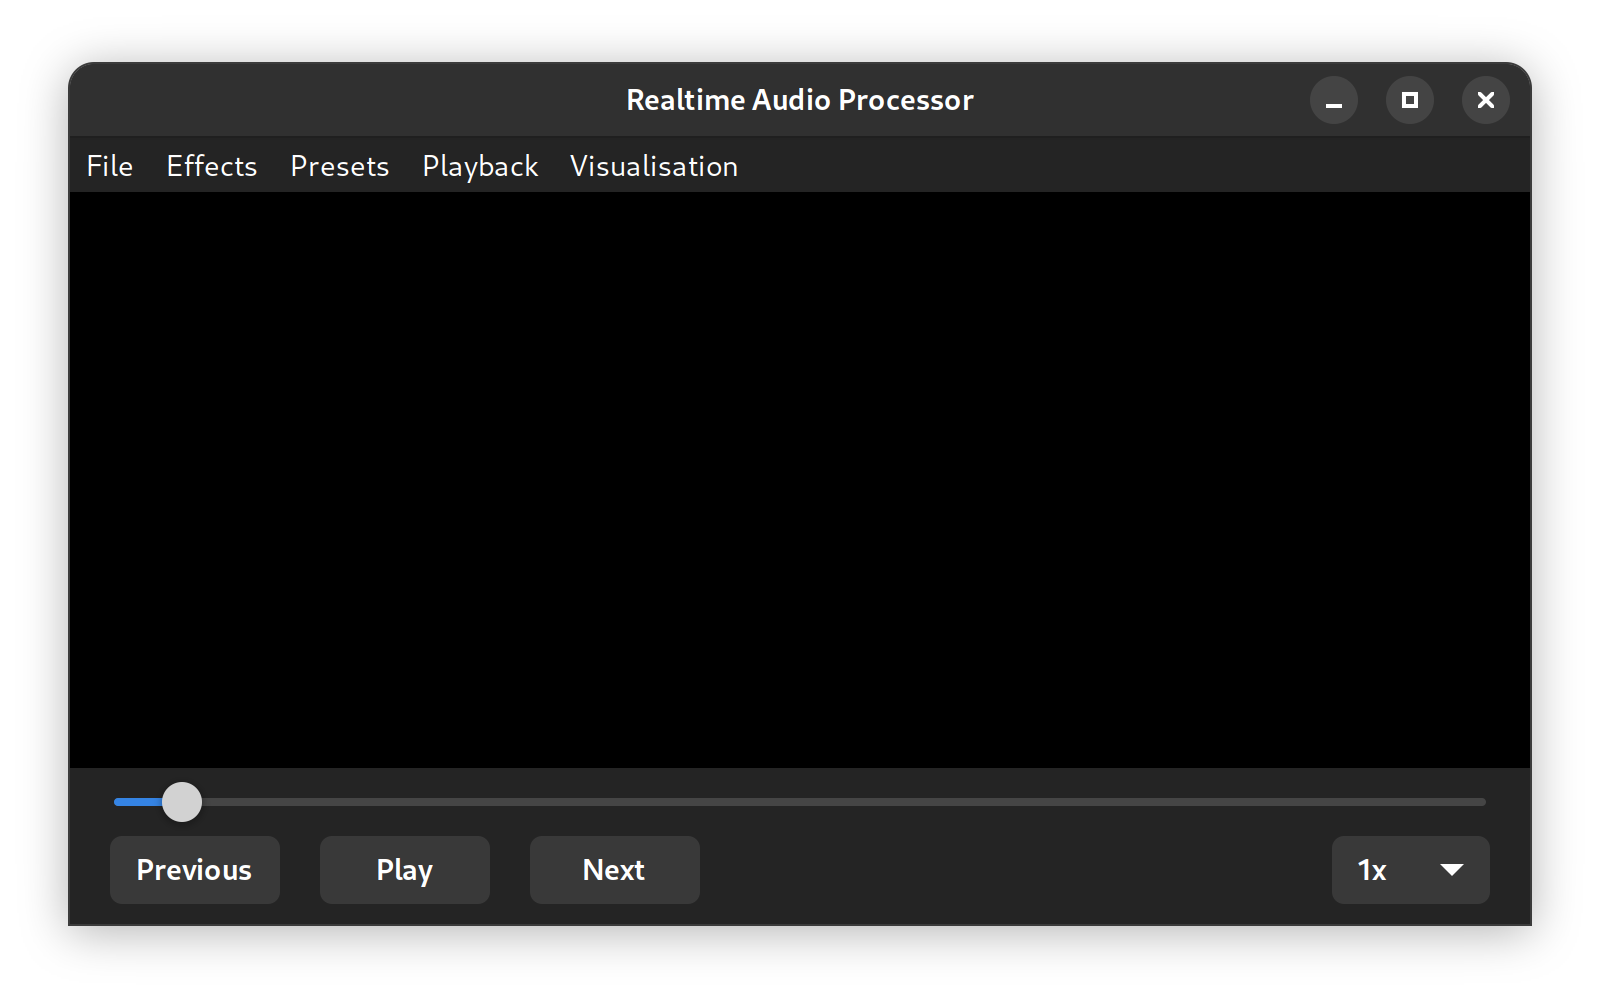
\includegraphics[width=14cm]{./tests/2.3.png}
\end{figure}

\subsubsection*{Conclusion}
A correct visualisation was achieved. The test was successful.

\pagebreak
\subsection{Test 2.4}
\subsubsection*{Description}
\paragraph{}
{
	\centering
	\fbox{\begin{minipage}{15cm}
			"A correct visualisation of two sine waves (one at 1,000 Hz and one at 10,000 Hz) is apparent, with two separate peaks corresponding to those frequencies."
	\end{minipage}}
}

\subsubsection*{Supplied Test Data}
An audio file consisting of two sine waves (at 1,000 Hz and 10,000 Hz respectively) was generated using the popular audio editing program Audacity.

\subsubsection*{Expected Result}
The visualiser should display two peaks, one to the right of the other. Recall that the x-axis is non-linear as it uses the Bark scale, so they will not be a "linear" distance apart.

\subsubsection*{Observed Result}
\label{sec:evidence2.4}
\begin{figure}[H]
	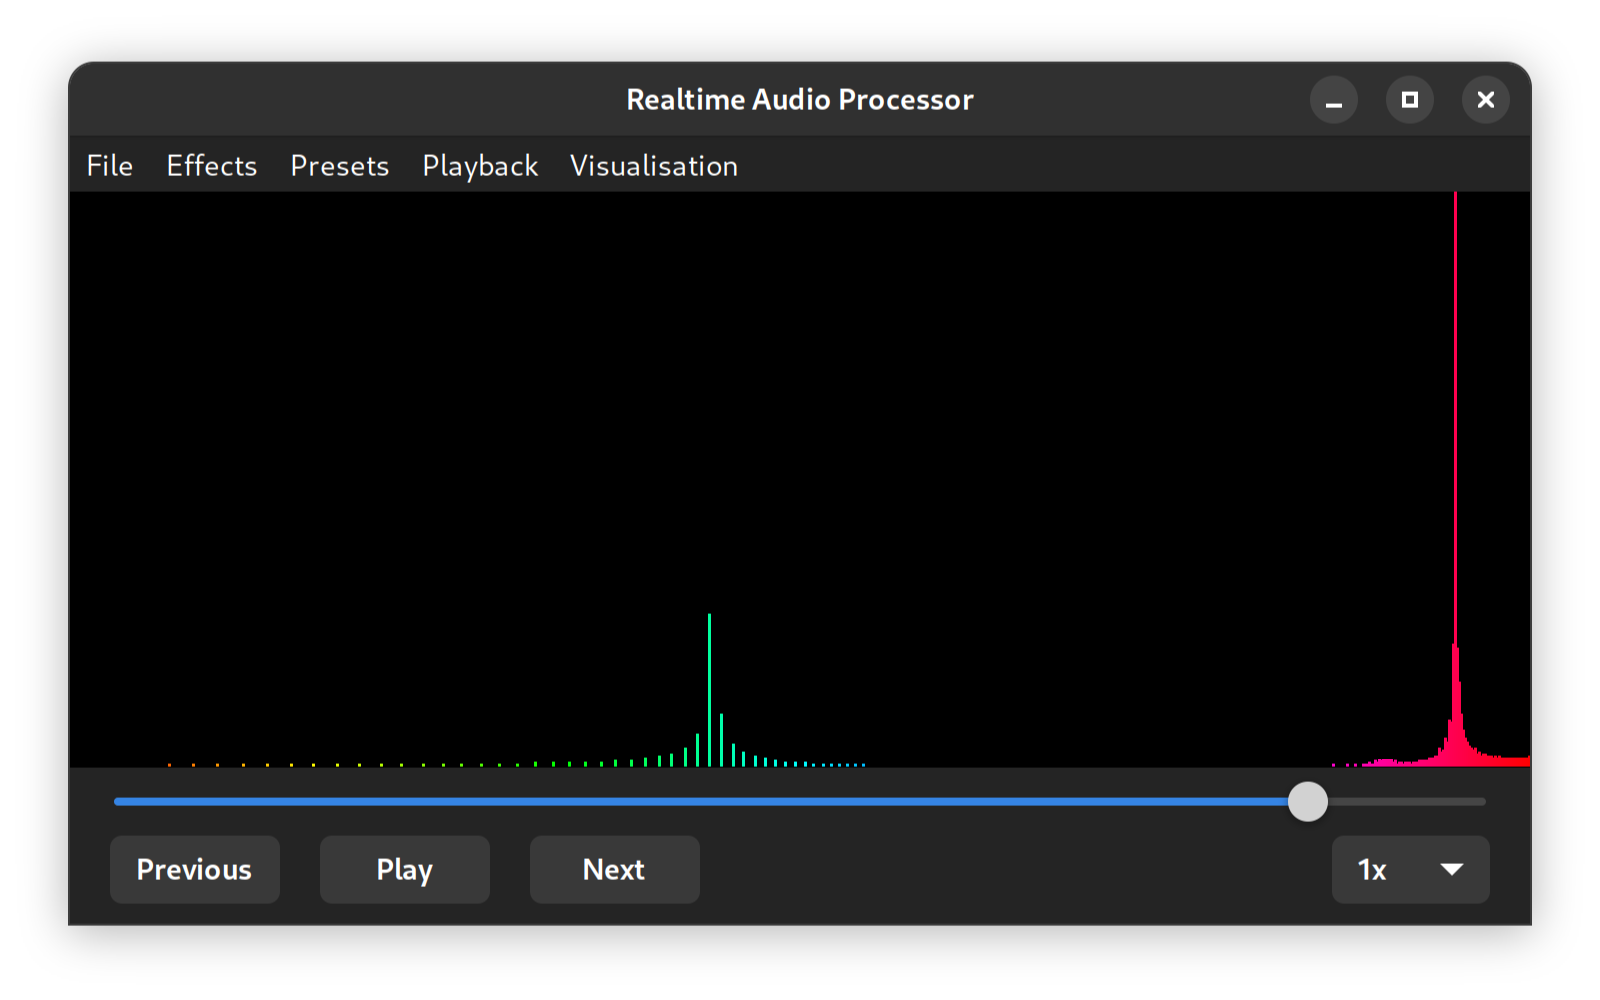
\includegraphics[width=14cm]{./tests/2.4.png}
\end{figure}

\subsubsection*{Conclusion}
A correct visualisation was achieved. The test was successful.


\pagebreak
\subsection{Test 2.5}
\subsubsection*{Description}
\paragraph{}
{
	\centering
	\fbox{\begin{minipage}{15cm}
			"A correct visualisation of three sine waves (1,000 Hz, 5,000 Hz and 15,000 Hz ) is apparent, with three separate peaks corresponding to those frequencies."
	\end{minipage}}
}

\subsubsection*{Supplied Test Data}
An audio file consisting of three sine waves (at 1,000 Hz and 5,000 Hz and 15,000 Hz respectively) was generated using the popular audio editing program Audacity.

\subsubsection*{Expected Result}
The visualiser should display three peaks in successive order. Recall that the x-axis is non-linear as it uses the Bark scale, so they will not be a "linear" distance apart.

\subsubsection*{Observed Result}
\label{sec:evidence2.5}
\begin{figure}[H]
	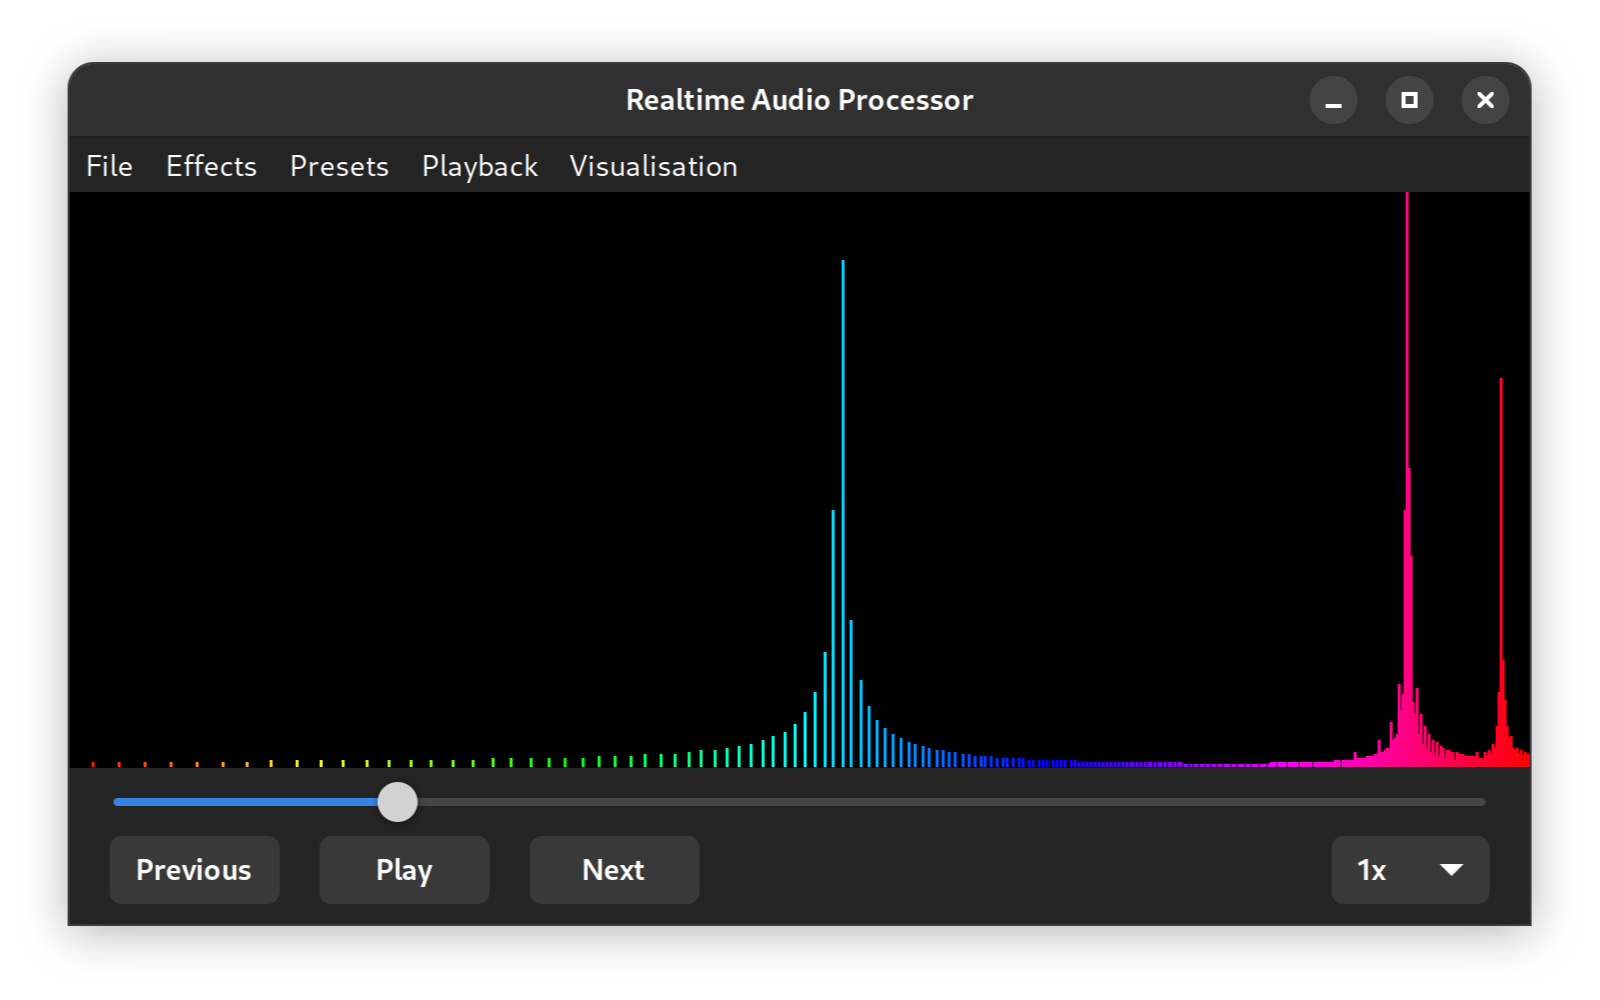
\includegraphics[width=14cm]{./tests/2.5.png}
\end{figure}

\subsubsection*{Conclusion}
A correct visualisation was achieved. The test was successful.


\pagebreak
\subsection{Test 3.1}
\subsubsection*{Description}
\paragraph{}
{
	\centering
	\fbox{\begin{minipage}{15cm}
			"The program's equaliser effect is able to selectively reduce the bass of any given audio (corresponding to the low frequencies in frequency space)."
	\end{minipage}}
}

\subsubsection*{Supplied Test Data}
Two songs are to be chosen as audio files, representative of the type of music often remixed (recall that the aim of the software is to assist in the creation of said remixes), both of which include ample bass. The "reduce bass" effects preset is to be applied within the software, which applies the "equaliser effect" with the correct parameters.

\subsubsection*{Expected Result}
To the human ear, the bass of the music (that is, the lower frequencies) should sound significantly reduced. This will be verified by observing the audio visualisation - the frequencies to the left should appear smaller in relation to the others.

\subsubsection*{Observed Result}
\label{sec:evidence3.1}
Video evidence was recorded for the test, which can be viewed \href{https://drive.google.com/file/d/1L1xcLyDd0HwsidX003OvKTqvFeIy20RA/view?usp=sharing}{here}\footnote{
	https://drive.google.com/file/d/1L1xcLyDd0HwsidX003OvKTqvFeIy20RA/view?usp=sharing
}. It shows the two songs being played first without the configured equaliser effect, then with the configured equaliser effect, then without again to highlight the contrast. Both songs have their bass almost completely eliminated, showcasing the effect at work. This is also visually demonstrated by the marked difference in the audio visualisation.

\subsubsection*{Conclusion}
The correct auditory effect was achieved, rendering the test successful.


\pagebreak
\subsection{Test 3.2}
\subsubsection*{Description}
\paragraph{}
{
	\centering
	\fbox{\begin{minipage}{15cm}
			"The program's equaliser effect is able to selectively reduce the treble of any given audio (corresponding to the high frequencies in frequency space)."
	\end{minipage}}
}

\subsubsection*{Supplied Test Data}
Two songs are to be chosen as audio files, representative of the type of music often remixed (recall that the aim of the software is to assist in the creation of said remixes), both of which include ample treble. The "reduce treble" effects preset is to be applied within the software, which applies the "equaliser effect" with the correct parameters.

\subsubsection*{Expected Result}
To the human ear, the treble of the music (that is, the higher frequencies) should sound significantly reduced. This will be verified by observing the audio visualisation - the frequencies in the middle should appear smaller in relation to the others.

\subsubsection*{Observed Result}
\label{sec:evidence3.2}
Video evidence was recorded for the test, which can be viewed \href{https://drive.google.com/file/d/1TrEiFpsmVm_sFzlnQu5FE8u7NDuP0Aq8/view?usp=sharing}{here}\footnote{
	https://drive.google.com/file/d/1TrEiFpsmVm\_sFzlnQu5FE8u7NDuP0Aq8/view?usp=sharing
}. It shows the two songs being played first without the configured equaliser effect, then with the configured equaliser effect, then without again to highlight the contrast. Both songs have their treble almost completely eliminated, showcasing the effect at work. This is also visually demonstrated by the marked difference in the audio visualisation.

\subsubsection*{Conclusion}
The correct auditory effect was achieved, rendering the test successful.


\pagebreak
\subsection{Test 4.1}
\subsubsection*{Description}
\paragraph{}
{
	\centering
	\fbox{\begin{minipage}{15cm}
			"A select group from the target audience certify that the echo effect sounds physically plausible, and mimics the effect as it is commonly heard in song remixes"
	\end{minipage}}
}

\subsubsection*{Supplied Test Data}
Two songs are to be chosen as audio files, representative of the type of music often remixed (recall that the aim of the software is to assist in the creation of said remixes). The audio effect will then be applied.

\subsubsection*{Expected Result}
There should be a noticeable echo to the audio. The "select group" will verify that the effect sounds correct (see description).

\subsubsection*{Observed Result}
\label{sec:evidence4.1}
Video evidence was recorded for the test, which can be viewed \href{https://drive.google.com/file/d/1gruw9Kz-T_HaHWCElk-2qzacudPEORu2/view?usp=sharing}{here}\footnote{
	https://drive.google.com/file/d/1gruw9Kz-T\_HaHWCElk-2qzacudPEORu2/view?usp=sharing
}. It shows the two songs being played first without the echo effect, then with the echo effect. An echo can clearly be heard.

\paragraph{Student 1 Response}
"There is certainly an echo in both songs that I can clearly hear, and I think it sounds very similar to the echoes I sometimes hear when a song's been modified. It's completely what I would expect."

\paragraph{Student 2 Response}
"Yes that's exactly what I thought I would hear. The effect is moderate but I understand it can be configured."

\paragraph{Student 3 Response}
"Your program has added an echo to songs like I thought [it would]. When people add echoes to remixes, this is what it sounds like."

\paragraph{Subject Specialist Response}
"Your echo effect sounds physically plausible for audio being played in a large room in which reflections attenuate little (e.g. a large hall or an outdoor venue). I believe it is therefore correct for the vast majority of situations. Obviously in situations where the audio is far away higher frequencies would be dampened significantly, but by combining the echo with your "equaliser" effect your software could achieve that too. So overall all types of echoes in the real-world can be effectively simulated with your project."

\subsubsection*{Conclusion}
An echo was clearly heard, which was certified by the select group as both the expected behaviour and physically plausible. The test passed.


\pagebreak
\subsection{Test 4.2}
\subsubsection*{Description}
\paragraph{}
{
	\centering
	\fbox{\begin{minipage}{15cm}
			"A select group from the target audience certify that the noise effect sounds physically plausible, and mimics the effect as it is commonly heard in song remixes"
	\end{minipage}}
}

\subsubsection*{Supplied Test Data}
Identical to test 4.1.

\subsubsection*{Expected Result}
There should be a noticeable noise within the audio. The "select group" will verify that the effect sounds correct (see description).

\subsubsection*{Observed Result}
\label{sec:evidence4.2}
Video evidence was recorded for the test, which can be viewed \href{https://drive.google.com/file/d/10Mj83b7_3bSNBfDXyYa7gKsn7GpRTCkY/view?usp=sharing}{here}\footnote{
	https://drive.google.com/file/d/10Mj83b7\_3bSNBfDXyYa7gKsn7GpRTCkY/view?usp=sharing
}. It shows the two songs being played first without the noise effect, then with the noise effect. Noise can clearly be heard.

\paragraph{Student 1 Response}
"I always hear this type of noise added to Lo-Fi remixes on YouTube, and it sounds just like that. I think your audio effect is perfect."

\paragraph{Student 2 Response}
"That's exactly what I meant to hear."

\paragraph{Student 3 Response}
"Yes, I think your noise effect is working as it should. It sounds correct."

\paragraph{Subject Specialist Response}
"The noise effect mimics the type of 'white noise' often picked-up by poor quality microphones (in which all frequencies are more-or-less represented), so I would indeed say your software project has resulted in a physically plausible noise."

\subsubsection*{Conclusion}
Noise in the audio was clearly heard, which was certified by the select group as both the expected behaviour and physically plausible. The test passed.


\pagebreak
\subsection{Test 4.3}
\subsubsection*{Description}
\paragraph{}
{
	\centering
	\fbox{\begin{minipage}{15cm}
			"The volume effect can be seen to adjust the volume correctly"
	\end{minipage}}
}

\subsubsection*{Supplied Test Data}
Identical to test 4.1. The volume effect is to be applied in an effort to reduce the volume.

\subsubsection*{Expected Result}
The audio should sound quieter.

\subsubsection*{Observed Result}
\label{sec:evidence4.3}
Video evidence was recorded for the test, which can be viewed \href{https://drive.google.com/file/d/1pJIc7vPbLUx2QlaXG3CymtYv7scC_tCX/view?usp=sharing}{here}\footnote{
	https://drive.google.com/file/d/1pJIc7vPbLUx2QlaXG3CymtYv7scC\_tCX/view?usp=sharing
}. It shows the two songs being played with the volume effect being used to change the volume. A change in volume can clearly be heard.

\subsubsection*{Conclusion}
A change in volume was clearly heard. The test passed.


\pagebreak
\subsection{Test 5.1}
\subsubsection*{Description}
\paragraph{}
{
	\centering
	\fbox{\begin{minipage}{15cm}
			" The noise effect can have its various parameters modified, which results in a correct change in the audio playback."
	\end{minipage}}
}

\subsubsection*{Supplied Test Data}
An audio file will be played and the intensity of the noise altered.

\subsubsection*{Expected Result}
The noise should vary in volume.

\subsubsection*{Observed Result}
\label{sec:evidence5.1}
Video evidence was recorded for the test, which can be viewed \href{https://drive.google.com/file/d/1Y1XaqZrhmlMwfaPEDRW-oboNUYbVYuxs/view?usp=drive_link}{here}\footnote{
	https://drive.google.com/file/d/1Y1XaqZrhmlMwfaPEDRW-oboNUYbVYuxs/view?usp=drive\_link
}.

\subsubsection*{Conclusion}
A change in the volume of the noise was clearly heard. The test passed.


\pagebreak
\subsection{Test 5.2}
\subsubsection*{Description}
\paragraph{}
{
	\centering
	\fbox{\begin{minipage}{15cm}
			" The echo effect can have its various parameters modified, which results in a correct change in the audio playback."
	\end{minipage}}
}

\subsubsection*{Supplied Test Data}
An audio file will be played and the echo's duration (how delayed the echo is) and fall-off (how quickly successive echoes reduce in volume) will be altered.

\subsubsection*{Expected Result}
The duration and fall-off of the echo should clearly be heard to change.

\subsubsection*{Observed Result}
\label{sec:evidence5.2}
Video evidence was recorded for the test, which can be viewed \href{https://drive.google.com/file/d/1XVe7SpYpZMCmoV4CvooNK1E8rbBCmQCn/view?usp=drive_link}{here}\footnote{
	https://drive.google.com/file/d/1XVe7SpYpZMCmoV4CvooNK1E8rbBCmQCn/view?usp=drive\_link
}.

\subsubsection*{Conclusion}
The observed results were in-line with what was expected. The test passed.


\pagebreak
\subsection{Test 5.3}
\subsubsection*{Description}
\paragraph{}
{
	\centering
	\fbox{\begin{minipage}{15cm}
			" The equaliser effect can have its various parameters modified, which results in a correct change in the audio playback."
	\end{minipage}}
}

\subsubsection*{Supplied Test Data}
An audio file will be played and the lower and upper frequency of the equaliser effect will be adjusted, in addition to the intensity of the effect.

\subsubsection*{Expected Result}
The range of frequencies targeted by the equaliser effect should vary, and the degree to which it is applied should clearly change.

\subsubsection*{Observed Result}
\label{sec:evidence5.3}
Video evidence was recorded for the test, which can be viewed \href{https://drive.google.com/file/d/1KebAYMMi3lstsluiX7-tS3c5MKMSElBV/view?usp=drive_link}{here}\footnote{
	https://drive.google.com/file/d/1KebAYMMi3lstsluiX7-tS3c5MKMSElBV/view?usp=drive\_link
}.

\subsubsection*{Conclusion}
The observed results were in-line with what was expected. The test passed.


\pagebreak
\subsection{Test 5.4}
\subsubsection*{Description}
\paragraph{}
{
	\centering
	\fbox{\begin{minipage}{15cm}
			" All presets present in the application can be loaded successfully, with the appropriate audio effects having been added and configured correctly, such that the desired effect is reached."
	\end{minipage}}
}

\subsubsection*{Supplied Test Data}
An audio file will be played. Successive presets will be applied.

\subsubsection*{Expected Result}
Each preset should result in the desired effect applied. Please consult the design section for more in-depth descriptions of what each preset aims to achieve (and why). However, broadly speaking:
\begin{itemize}
	\item Spacious room - the audio sounds like it's in a spacious room (e.g. a large school sports hall)
	\item Far away room - the audio sounds like you're listening to it from far away
	\item Lo-fi - relaxing - the audio mimics the "Lo-fi" genre and is slowed down
	\item Lo-fi - energy - the audio mimics the "Lo-fi" genre and is sped up
	\item Remove bass - the audio has had its lower frequencies removed
	\item Remove treble - the audio has had its higher frequencies removed
	\item Low quality speakers - the audio sounds like it's coming from low-quality speakesr
\end{itemize}
Each preset should have set-up one or more audio effects configured correctly. Effects will be considered "configured correctly" if the desired artistic effect is achieved.

\subsubsection*{Observed Result}
\label{sec:evidence5.4}
Video evidence was recorded for the test, which can be viewed \href{}{here}\footnote{

}.

\subsubsection*{Conclusion}
The observed results were in-line with what was expected. The test passed.


\pagebreak
\subsection{Tests 6.1 and 6.2}
\subsubsection*{Descriptions}
\paragraph{}
{
	\centering
	\fbox{\begin{minipage}{15cm}
			\paragraph{Test 6.1} The program must run, without any effects applied, in real-time on the specified hardware.
			\paragraph{Test 6.2} The program must run in real-time, with every effect applied at once, in real-time on the specified hardware.
	\end{minipage}}
}

\subsubsection*{Supplied Test Data}
\paragraph{}
Recall that the hardware chosen was discussed in detail during the design section. In summary, to represent an average school computer I will use one at my school, which is representative of average high-school hardware. I will also use my personal school laptop (which is slightly less powerful). As I wish to identify the boundaries of my program's performance, I have also decided to run the performance tests on a very old laptop of mine from 2012, with a weak CPU from 2013. If it runs on this, it stands to reason that the tests are not only met but \textit{exceeded}, as the speed of this machine is far below what an average school computer of today would possess.  

\paragraph{}
As the software performs all processing on the CPU, the most important detail is the clock-speed. Recall that the software only uses two threads (one for the GUI, one for the audio), so core-counts higher than two are unlikely to affect performance.

\paragraph{}
Temporary timing code was added as discussed in the design section. In the \textit{OnPaint} subroutine under \textit{src/ui/audio\_visualiser.cpp}, which draws the visualisation\footnote{
	Recall that the actual computation / maths behind the visualisation are actually done on the audio-thread, so will be included under the timing of the audio callback ("audio processing").
} was modified as so:

\begin{minted}{c++}
#include <chrono>
#include <iostream>
	
void AudioVisualiser::OnPaint(const wxPaintEvent& event)
{
	using namespace std::chrono;
	const steady_clock::time_point begin = std::chrono::steady_clock::now();
	
	// rest of code
	
	const steady_clock::time_point end = std::chrono::steady_clock::now();
	const int64_t duration = duration_cast<std::chrono::nanoseconds>(end - begin).count();
	std::cout << "Audio processing took " << (float)duration / 1000000.0f << " ms" << std::endl;
}
\end{minted}

\pagebreak
\paragraph{}
The \textit{OnAudioCallback} subroutine under \textit{src/io/audio\_stream} was modified in much the same way:
\begin{minted}{c++}
	#include <chrono>
	#include <iostream>
	
	void AudioStream::OnAudioCallback(uint8_t* buffer, int length)
	{
		using namespace std::chrono;
		const steady_clock::time_point begin = std::chrono::steady_clock::now();
		
		// rest of code
		
		const steady_clock::time_point end = std::chrono::steady_clock::now();
		const int64_t duration = duration_cast<std::chrono::nanoseconds>(end - begin).count();
		std::cout << "Visual processing took " << (float)duration / 1000000.0f << " ms" << std::endl;
	}
\end{minted}

\subsubsection*{Expected Result}
All pieces of hardware, as discussed in the design section, must be able to process audio in under 3ms and update the visuals in less than 16.6ms.

\subsubsection*{Observed Result}
Below is a summary followed the relevant screenshots of the program's output.
{
	\renewcommand{\arraystretch}{1.5}
	\begin{table}[h!]
		\begin{center}
			\begin{tabularx}{1.0 \textwidth} {
					| >{\raggedright\arraybackslash}X
					| >{\raggedright\arraybackslash}X
					| >{\raggedright\arraybackslash}X
					| >{\raggedright\arraybackslash}X
					| >{\raggedright\arraybackslash}X
					| >{\raggedright\arraybackslash}X
					| >{\raggedright\arraybackslash}X
					|
				}
				\hline
				Test & Piece of Hardware & CPU & CPU Frequency  & CPU core-count & Time to Update Audio & Time to Update Visuals \\
				
				\hline
				6.1 & School computer &  &  &  & 0.02ms & 1-3ms \\
				
				\hline
				6.2 & School computer & & & & 0.7-1.1ms & 2-4ms \\
				
				\hline
				6.1 & Personal school laptop & Intel i5-7Y540 & 3.2 GHz & 2 & 0.02ms & 2-5ms \\
				
				\hline
				6.2 & Personal school laptop & Intel i5-7Y540 & 3.2 GHz & 2 & 1.0ms & 2-4ms \\
				
				\hline
				6.1 & Very old laptop & Intel i5-4258U & 2.4 GHz & 2 & 1ms & 10-13ms \\
				
				\hline
				6.2 & Very old laptop & Intel i5-4258U & 2.4 GHz & 2 & 2.1-2.8ms & 11-13ms \\
				
				\hline
			\end{tabularx}
		\end{center}
	\end{table}
}

\label{sec:evidence6}
\begin{figure}[H]
	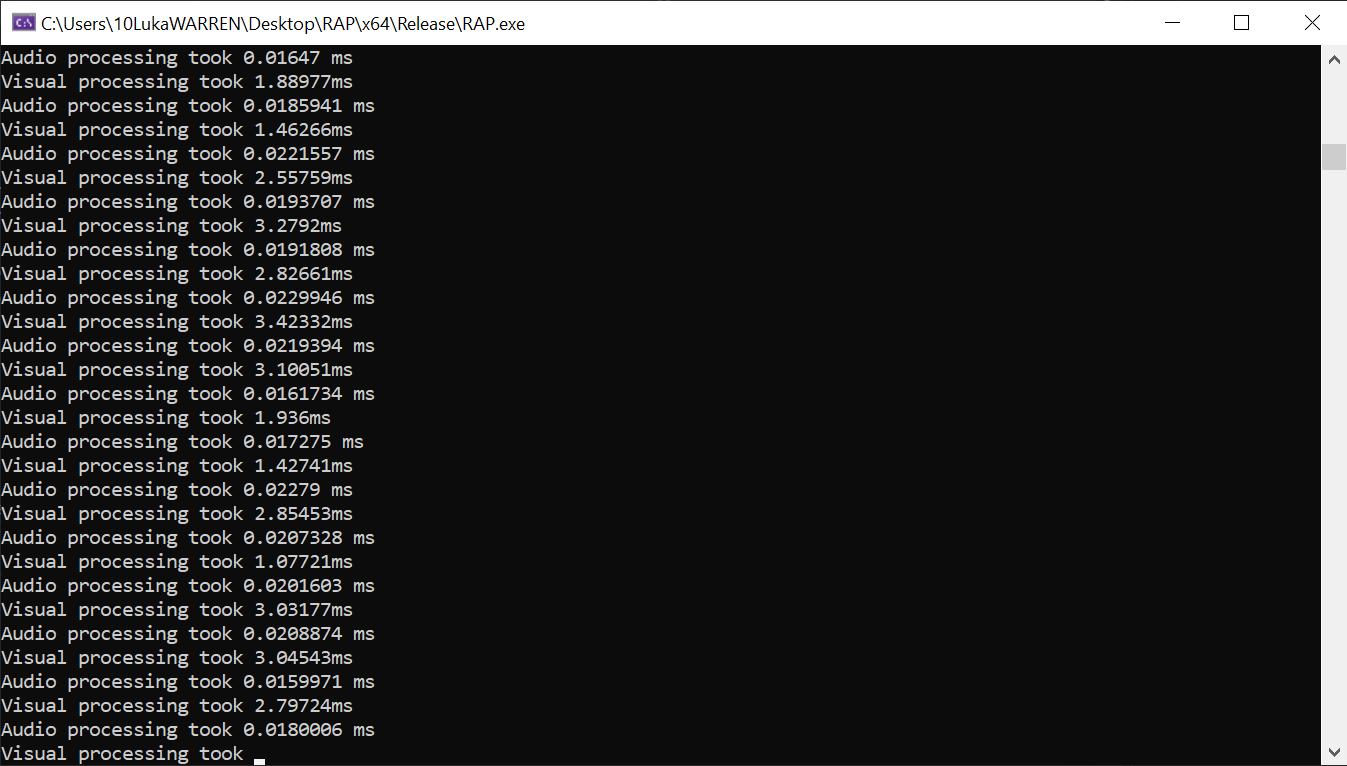
\includegraphics[width=14cm]{./tests/6.1 school computer.png}
	\caption{Test 6.1 performance capture screenshot for "school computer"}
\end{figure}
\begin{figure}[H]
	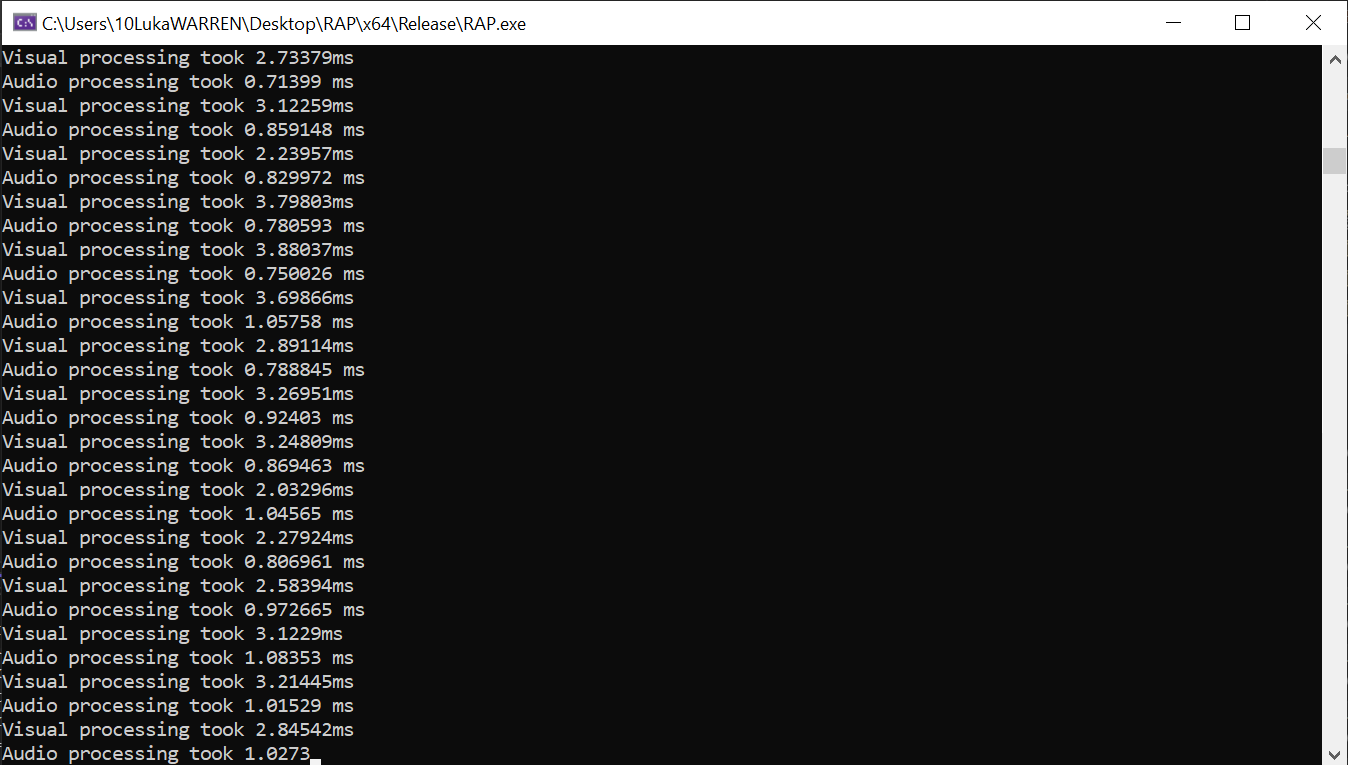
\includegraphics[width=14cm]{./tests/6.2 school computer.png}
	\caption{Test 6.2 performance capture screenshot for "school computer"}
\end{figure}
\begin{figure}[H]
	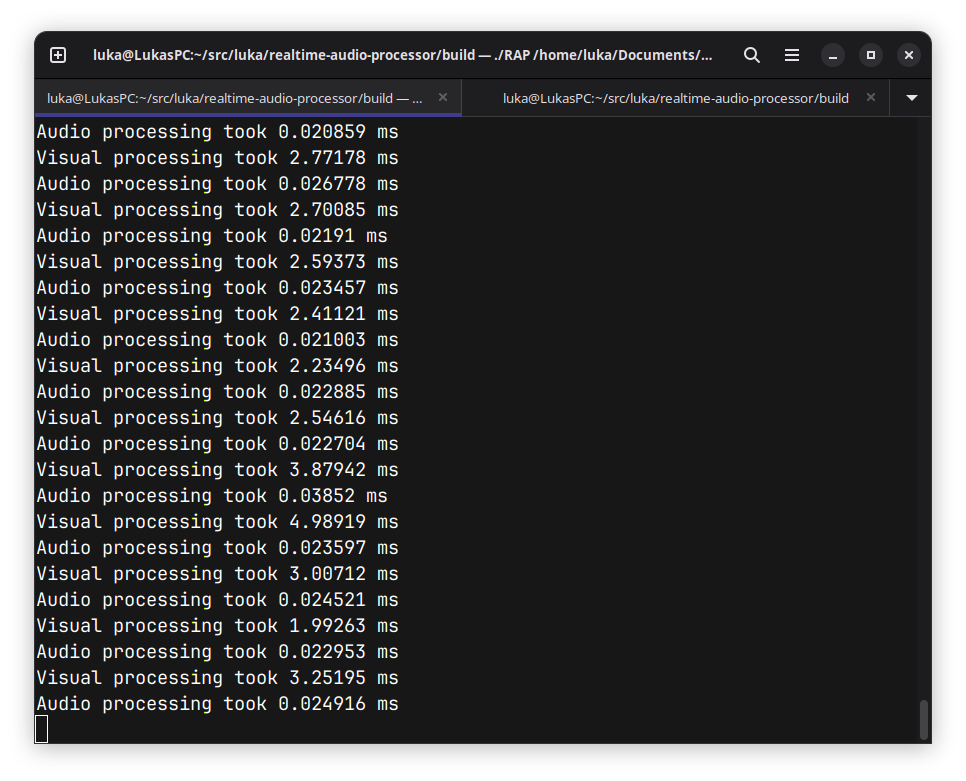
\includegraphics[width=14cm]{./tests/6.1 laptop.png}
	\caption{Test 6.1 performance capture screenshot for "personal school laptop"}
\end{figure}
\begin{figure}[H]
	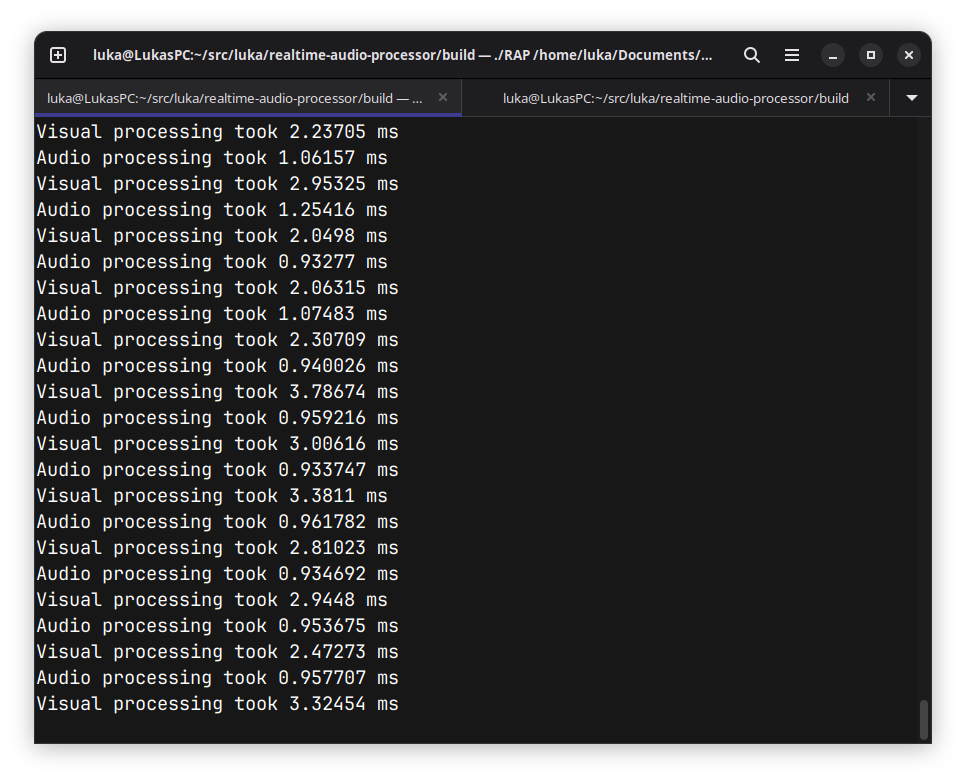
\includegraphics[width=14cm]{./tests/6.2 laptop.png}
	\caption{Test 6.2 performance capture screenshot for "personal school laptop"}
\end{figure}
\begin{figure}[H]
	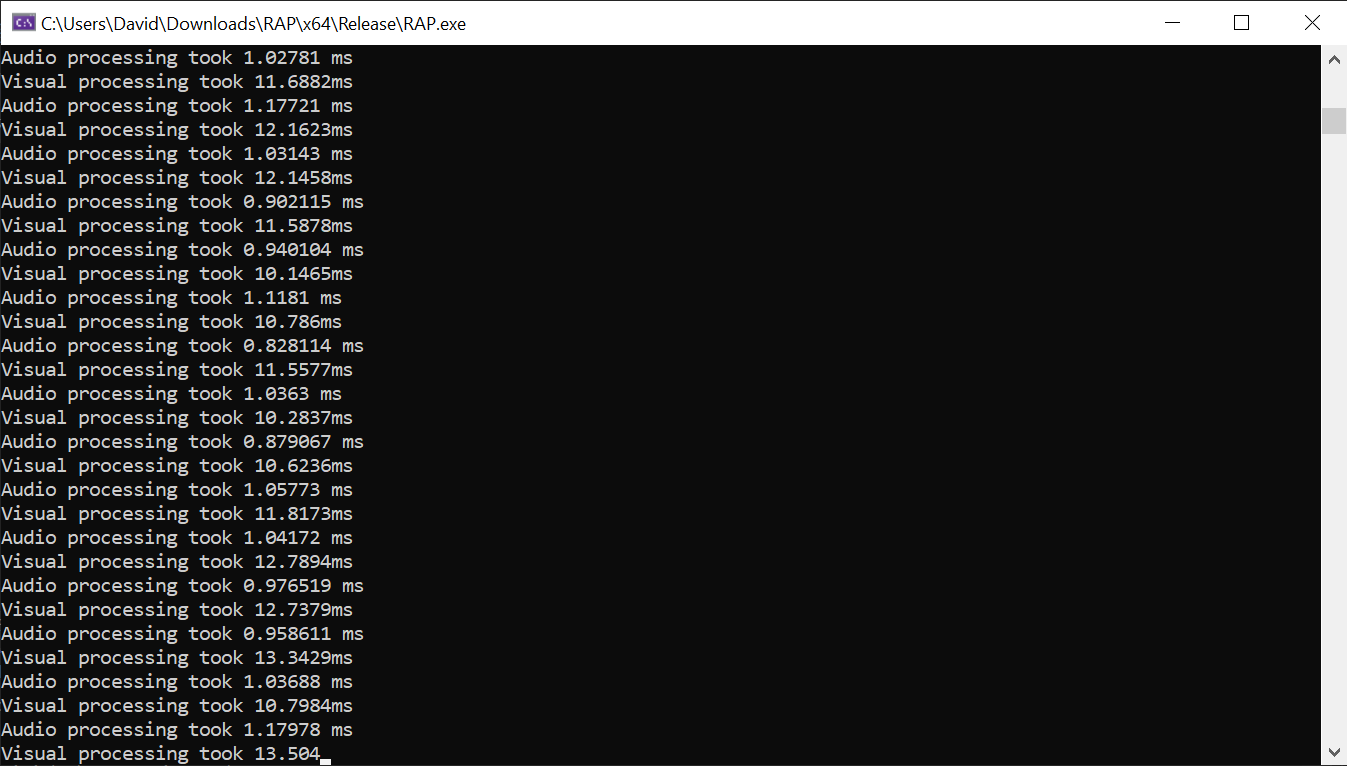
\includegraphics[width=14cm]{./tests/6.1 old laptop.png}
	\caption{Test 6.1 performance capture screenshot for "very old laptop"}
\end{figure}
\begin{figure}[H]
	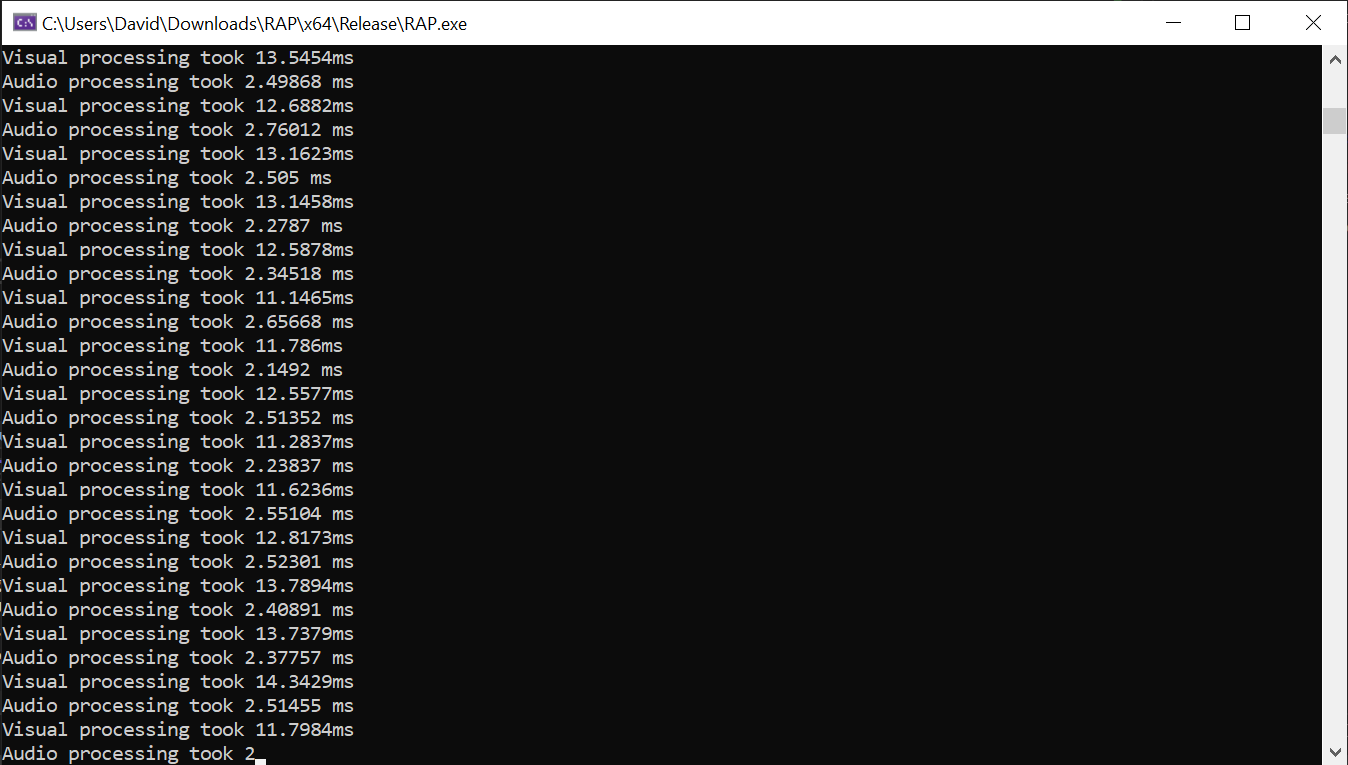
\includegraphics[width=14cm]{./tests/6.2 old laptop.png}
	\caption{Test 6.2 performance capture screenshot for "very old laptop"}
\end{figure}

\subsubsection*{Conclusion}
All hardware samples were able to meet the "real-time" criteria for both tests 6.1 and 6.2. Even the "very old laptop", with a CPU from 2013, was able to just about stay under the performance targets set. As a result, I can say with confidence that the test was not only met but \textit{exceeded}, as performance was actually better than required. 